\documentclass[12pt]{article}
\usepackage[utf8]{inputenc}
\usepackage{multicol}
\usepackage{graphicx}
\usepackage{subfig}
\usepackage{listings}
\usepackage{caption}
%\usepackage[backend=biber,style=authoryear]{biblatex}
\usepackage[margin=1in]{geometry}
\usepackage[toc,page]{appendix}
%\addbibresource{bibliography.bib}
\usepackage{indentfirst}
\usepackage{amsmath}
\usepackage{setspace}
\usepackage{etoolbox}
\usepackage{array}
\usepackage{chngcntr}

\usepackage{tocloft}
\renewcommand{\cftsecleader}{\cftdotfill{\cftdotsep}}



\usepackage[utf8]{inputenc}
\usepackage[english]{babel}
\usepackage[backend=biber,style=alphabetic, sorting=ynt]{biblatex}
\addbibresource{bibliography.bib}
\bibliographystyle{apalike}

\counterwithin{table}{section}
\counterwithout{figure}{section}
\newcolumntype{P}[1]{>{\centering\arraybackslash}p{#1}}
\graphicspath{ {thesis/images/} }
\makeatletter
\pretocmd{\@sect}{\singlespacing}{}{}
\pretocmd{\@ssect}{\singlespacing}{}{}
\apptocmd{\@sect}{\doublespacing}{}{}
\apptocmd{\@ssect}{\doublespacing}{}{}
\makeatother


\doublespacing

\begin{document}
%------------------------Title Page----------------------------------------

\begin{titlepage}
	\begin{center}
		
		\normalsize
		\textbf{CLASSIFYING  WEBSITES  USING  WORD  VECTORS  AND  OTHER  TECHNIQUES:}\\
		\medskip
		\textbf{AN APPLICATION OF ZIPF'S LAW}
		
		\vspace{2.1cm}
		
		A THESIS \\
		\medskip
		Presented to the Department of Applied Statistics \\
		\medskip
		California State University, Long Beach
		
		\vspace{2.2cm}
		
		In Partial Fulfillment\\
		\medskip
		of the Requirements for the Degree\\
		\medskip
		Master of Science in Applied Statistics
		
		\vspace{2.2cm}
		
		Committee Members:\\
		\medskip
		Kagba Suaray, Ph.D. (Chair)\\
		Wenlu Zhang, Ph.D.\\
		James VonBrecht, Ph.D.\\
		\medskip
		College Designee:\\
		\medskip
		Tangan Gao, Ph.D.
		
		\vfill
		
		By Alejandro Robles\\
		\medskip
		B.S., 2016, University of California, Los Angeles\\
		\medskip
		July 2019
		
		
	\end{center}
\end{titlepage}
%----------------------ABSTRACT----------------------------

\begin{center}
\section*{ABSTRACT}
\end{center}
%{\normalfont ABSTRACT}


In this paper, we explore the effectiveness of using Zipf's Law as a pre-processing step for classifying websites into four categories: Sports, Games \& Toys, Travel, and Food \& Drink. The classifiers used were Multinomial Logistic Regression  and Convolutional Neural Network (CNN) using Glove word embeddings. The CNN with Glove embeddings as input produces 92\% accuracy but increases to 93\% when applying Zipf's Law. The worst performing was the logistic regression with Glove embeddings with accuracy of 90\%. After we transformed our multiclass classification problem into a binary one, we saw a jump in accuracy. All models got an accuracy of 94\% except for the base model (TF-IDF \& LOGIT), which got a 93\% accuracy.

All the code can be found on github.com\footnote{\url{https://github.com/alejandro-robles7/Thesis}}.

\renewcommand{\thepage}{\roman{page}}
\setcounter{page}{2}

\newpage

%------------------------Table of Contents---------------------------------
\renewcommand\contentsname{\begin{center}
TABLE OF CONTENTS
\end{center}
}
\setcounter{tocdepth}{1}

\tableofcontents
\addcontentsline{toc}{section}{ABSTRACT}

%\addcontentsline{toc}{section}{INTRODUCTION AND DATA SET}

\addcontentsline{toc}{section}{LIST OF TABLES}

\addcontentsline{toc}{section}{LIST OF FIGURES}

\addcontentsline{toc}{section}{     \normalfont{Introduction}}





\newpage
\renewcommand\listtablename{\begin{center}LIST OF TABLES\end{center}}
%\addcontentsline{toc}{section}{LIST OF TABLES}
\listoftables

\newpage
\renewcommand\listfigurename{\begin{center}LIST OF FIGURES\end{center}}
%\addcontentsline{toc}{section}{LIST OF FIGURES}
\listoffigures



\newpage

%------------------------LITERATURE REVIEW---------------------------------
\renewcommand{\thepage}{\arabic{page}}
\setcounter{page}{1}

%\section{Introduction and Data Set}
%\section{Introduction and Data Set}
%\section*{\begin{center}CHAPTER 1 \newline INTRODUCTION AND DATA SET \end{center}}


\section*{
\begin{center}
CHAPTER 1 
\end{center}
\newline 
\begin{center}
INTRODUCTION AND DATA SET
\end{center}
}

\addtocounter{section}{1}


\begin{center}
\subsection{Introduction}
\end{center}

Contextual advertising is a type of targeted advertising displayed on a diversity of mediums such as websites or mobile browsers. A system needs to scan for keywords found on a website's content to determine its category such as sports or travel. If an advertiser, company or person that advertises a product, is promoting new soccer gear, then it is in their interest to target users who visit sport's related sites. This is in essence contextual targeting.  With millions of websites online, it is not humanly possible to visit each website, read the content, and classify websites. Classifying websites based on their content is not a trivial task. Natural language processing (NLP) must be used to process website data, which is often unstructured data, to be able to build models from it. More generally, NLP helps us transform words and text into numerical vectors which is required to do mathematical modeling.

Text processing is a fundamental step when building a text classifier. Simply put, text processing is transforming text so that it is predictable and analyzable for one's task. This includes removing noise. Noise can be defined as text that adds no valuable information to the classification algorithm. For example, words such as "the", "in", or "a" are very common words that do not add any signal. These words are examples of stop words. Removing stop words, stemming and other NLP techniques, which we will cover in later chapters, must be applied to increase precision. This can be challenging when dealing with scraped websites because of text that is not reflective of content such as HTML tags and other text that is native to websites. Zipf's Law can be applied for preprocessing text. Word frequencies that follow a power law can use Zipf's law to segregate content in three sections : stop words, rare words, and words that reflect content \cite{Yatsko:2015:ATC:2813730.2813744}. By selecting only the latter, the accuracy of downstream machine learning applications should increase.

Feature extraction is another NLP process vital for downstream machine learning applications. Deriving fixed length values, features, that are informative and non-redundant for machine learning tasks from variable length text is a requirement. Vector Space Models (VSM) such as TF-IDF and word embeddings provide frameworks for performing feature extraction methods. VSMs objective is to create embeddings for documents, phrases, or words which maps them in a vector space such that semantically similar objects are close in distance \cite{Turney:2010:FMV:1861751.1861756}.

Classification algorithms are a type supervised learning. Generally, the input is data that is labeled into categories. Then using this ground truth, the model is trained to fit the data to be used for predicting labels for new observations. In our study, we use Multinomial Logistic Regression (MLOGIT) and one dimensional Convolutional Neural Network (CNN), which we will discuss in future chapters. 

Part of the motivation for this study was based on an experimental design previously conducted \cite{previous}. The two way factor anova with blocking effect tested which of the three factors, feature extraction, clustering algorithm, or language, contributed most to minimizing clustering error metrics. According to Robles (2018), feature extraction methods are the most influential step when clustering similar websites. This motivated research into more advanced feature extraction pipelines.

Building upon recent work \cite{previous2}, the objective of our project is to not only increase the accuracy of classifying websites but also generate meaningful embeddings for these websites by applying Zipf's law to pre-process the text. In short, we want to extend the results for word vectors generated by models such as skip-gram to websites and explore how Zipf's Law can help us identify text that reflects the content. Just like similar words are mapped close together, we are hoping that our URL embeddings will also map similar sites close in distance. If this is true, then downstream machine learning applications such as clustering or classifying sites will be greatly facilitated. 

To measure success we will classify sites into four categories using a common classifier such as multinomial logistc regression and a more complex CNN architecture model . We will test how different feature extraction methods affect accuracy. As a base, we will use TF-IDF to generate features for the sites. Then we will use GloVe word embeddings with and without Zipf's Law to see if this increases the accuracy. Finally, we visualize how the embeddings display semantic relationships. 

\begin{center}
\subsection{The Data Set}
\end{center}

This dataset was scraped from 12,874 websites in February of 2019. The dataset is all the text found on each of those websites. After cleaning the data 10,626 distinct websites remained. Cleaning the data included finding non-english text and removing those websites. Furthermore some websites did not contain any text so we also removed these instances from our dataset. After that we cleaned the text of the remaining websites. This included removing stop words, transforming all the text to lowercase and removing non-ASCII-characters.

Each of the 10,626 websites belongs to one of the categories "Sports", "Food \& Drink", "Games \& Toys", "Travel". We chose these four categories since they contain the biggest number of instances and least mutually similar. The distribution of instances across these four classes can be seen in Figure 1. Because the data is imbalanced, a classifier always predicting "Sports" will reach an accuracy of 46 \%.

The website with the greatest amount of words contains 44,801 words. On average, each website contains 678 words. The total number of words across all websites sums up to 7,200,956 words.

\begin{figure}[ht!]
\center
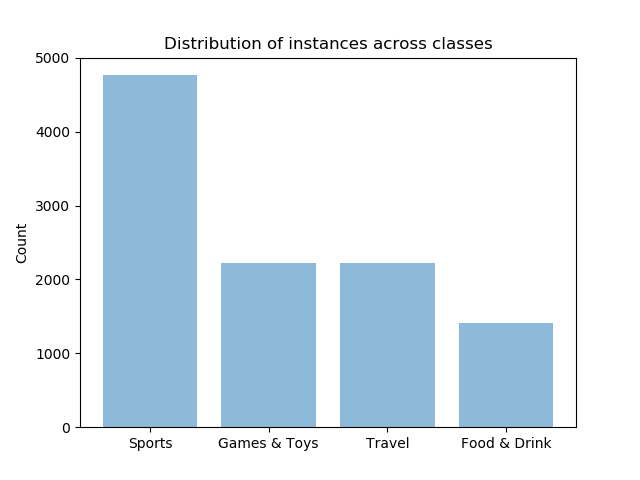
\includegraphics[width=90mm]{classes.png}
    \caption{Distribution of instances among classes}
    \label{instances_classes}
\end{figure}


\newpage

\section*{
\begin{center}
CHAPTER 2 
\end{center}
\newline 
\begin{center}
LITERATURE REVIEW
\end{center}}

\setcounter{subsection}{0}
\addtocounter{section}{1}

There exists numerous approaches to text classification. Researchers have used simple techniques such as bag of words, to hand crafted features, to more complex deep learning architectures to solve this issue. Text classification reach many domains such as social media, fiction novels, and search engines.  

\begin{center}
\subsection{Detecting Satire in the News with Machine Learning}
\end{center}


\cite{detect} used Logistic Regression and Support Vector Machines to classify websites to detect satire (fake news). They followed the sentiment behind \cite{Halevy:2009:UED:1525642.1525689} where he explains how more data has bigger impact on performance than better algorithms. To collect labeled data, they gathered news articles from both trusted and satirical publishers. Their data was relatively larger (63,868 article) compared to 480 articles used by \cite{Rubin:2015:DDN:2857070.2857153} . For text processing they also applied ``homogeneity in lengths'' where they removed articles that had less than 500 or more than 10,000 characters. For feature extraction, they opted with TF-IDF approach. Their results were an improvement to experiments with smaller data sets and similar to experiments with hand crafted features. This shows how with just more data they were able to have performing classifiers. They initially got a test accuracy of 99.6\% but they suspected that the algorithm was detecting different publishers as suppose to satire. To test this, they left out a publisher from each class for their training set and used them as test set. This new set up resulted in a 88.2\% accuracy.


\begin{center}
\subsection{A Naive Bayes approach for URL classification with supervised feature selection and rejection framework}
\end{center}


\cite{inbook} provides a framework to efficiently classify websites. Instead of immediately classifying websites based on scraped content, he first attempts to classify websites using only the Uniform Resource Locator's (URL) to generate features. By URL here we mean using "travel.com" as input instead of scraping the content of the website. This reduces the latency of classification. Additionally, they use a variant of chi-squared to do feature selection from features based on n-grams. First, they remove protocol information and terms such as ``www''. Then they create tokens by using special characters such as slash, dot, hyphens, and other characters as delimiters. So for example, the URL ``http://www.bl.uk/whats-on'' will have the following tokens: ``bl'', ``uk'', ``whats'', and ``on''. 

After tokenizing words, they use n-grams as a way to create features. Below is an illustration. Here n-grams means that for each token, we extract n-character length phrases.

\begin{verbatim}
URL: http://www.bl.uk/whats-on/
Tokens: bl, uk, whats, on
3-grams: wha, hat, ats
4-grams: what, hats
5-grams: whats
6-grams:
7-grams:
8-grams:
\end{verbatim}


Here they first concatenate the tokens and then apply n grams.

\begin{verbatim}
URL: http://www.bl.uk/whats-on/
Tokens: bl, uk, whats, on
Concatenated URL text: blukwhatson
3-grams: blu, luk, ukw, kwh, wha, hat, ats, tso, son
4-grams: bluk, lukw, ukwh, kwha, what, hats, atso, tson
5-grams: blukw, lukwh, ukwhat, kwhat, whats, hatso, atson
6-grams: blukwh, lukwha, ukwhat, kwhats, whatso, hatson
7-grams: blukwha, lukwhat, ukwhats, kwhatso, whatson
8-grams: blukwhat, lukwhats, ukwhatso, kwhatson
\end{verbatim}

\begin{figure}[ht!]
\center
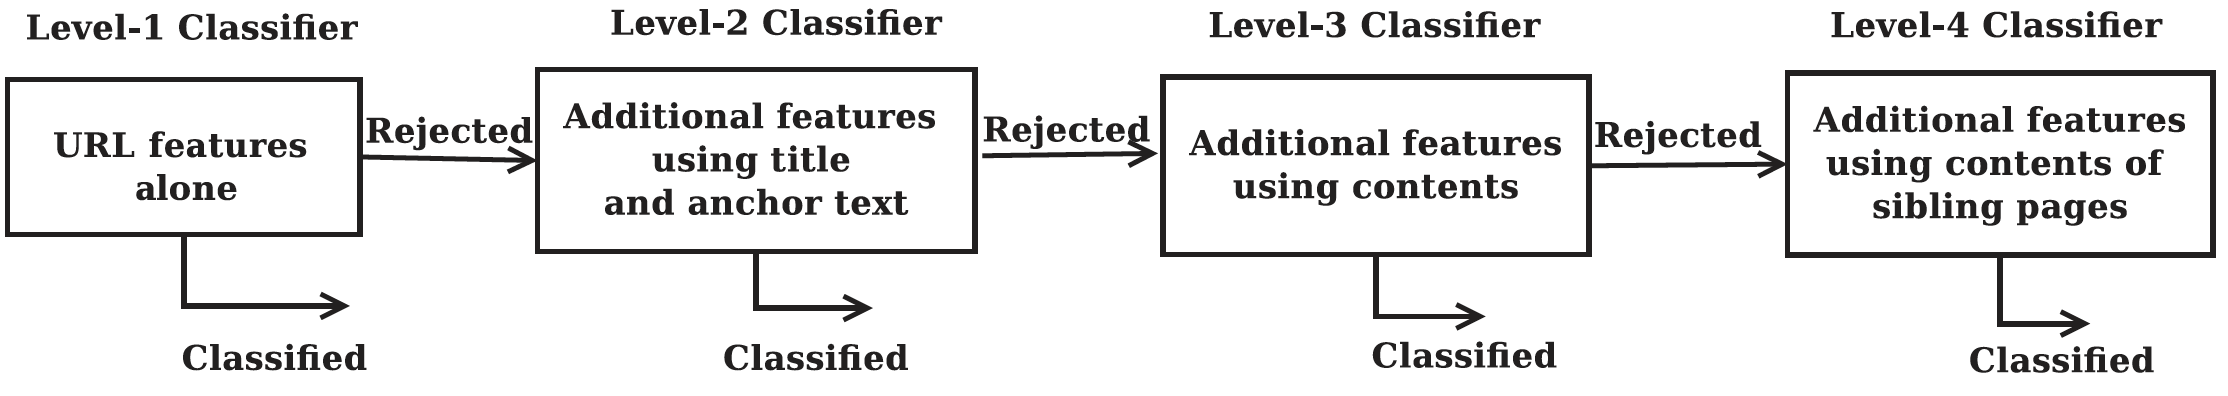
\includegraphics[width=130mm]{rejection_method.png}
    \caption{Multilevel classifier design. URL, uniform resource locator}
    \label{reject}
\end{figure}


The classification algorithm they choose is Naive Bayes. If the confidence score is less than a threshold then they avoid making any classifications. Instead they sequentially add more inputs until the confidence score is above the threshold starting with url features, then title and anchor, proceeding with more text content and finally using pages from the same domain. This can be seen in Figure \ref{reject} The multiclass accuracy of 70\% can be achieved by rejecting 30\% of URLs. As a first-level classifier using URL-based features, multiclass accuracy can be pushed up to 0.979. This is a trade off between rejection and accuracy as we can see in Figure \ref{reject_acc}.

\begin{figure}[ht!]
\center
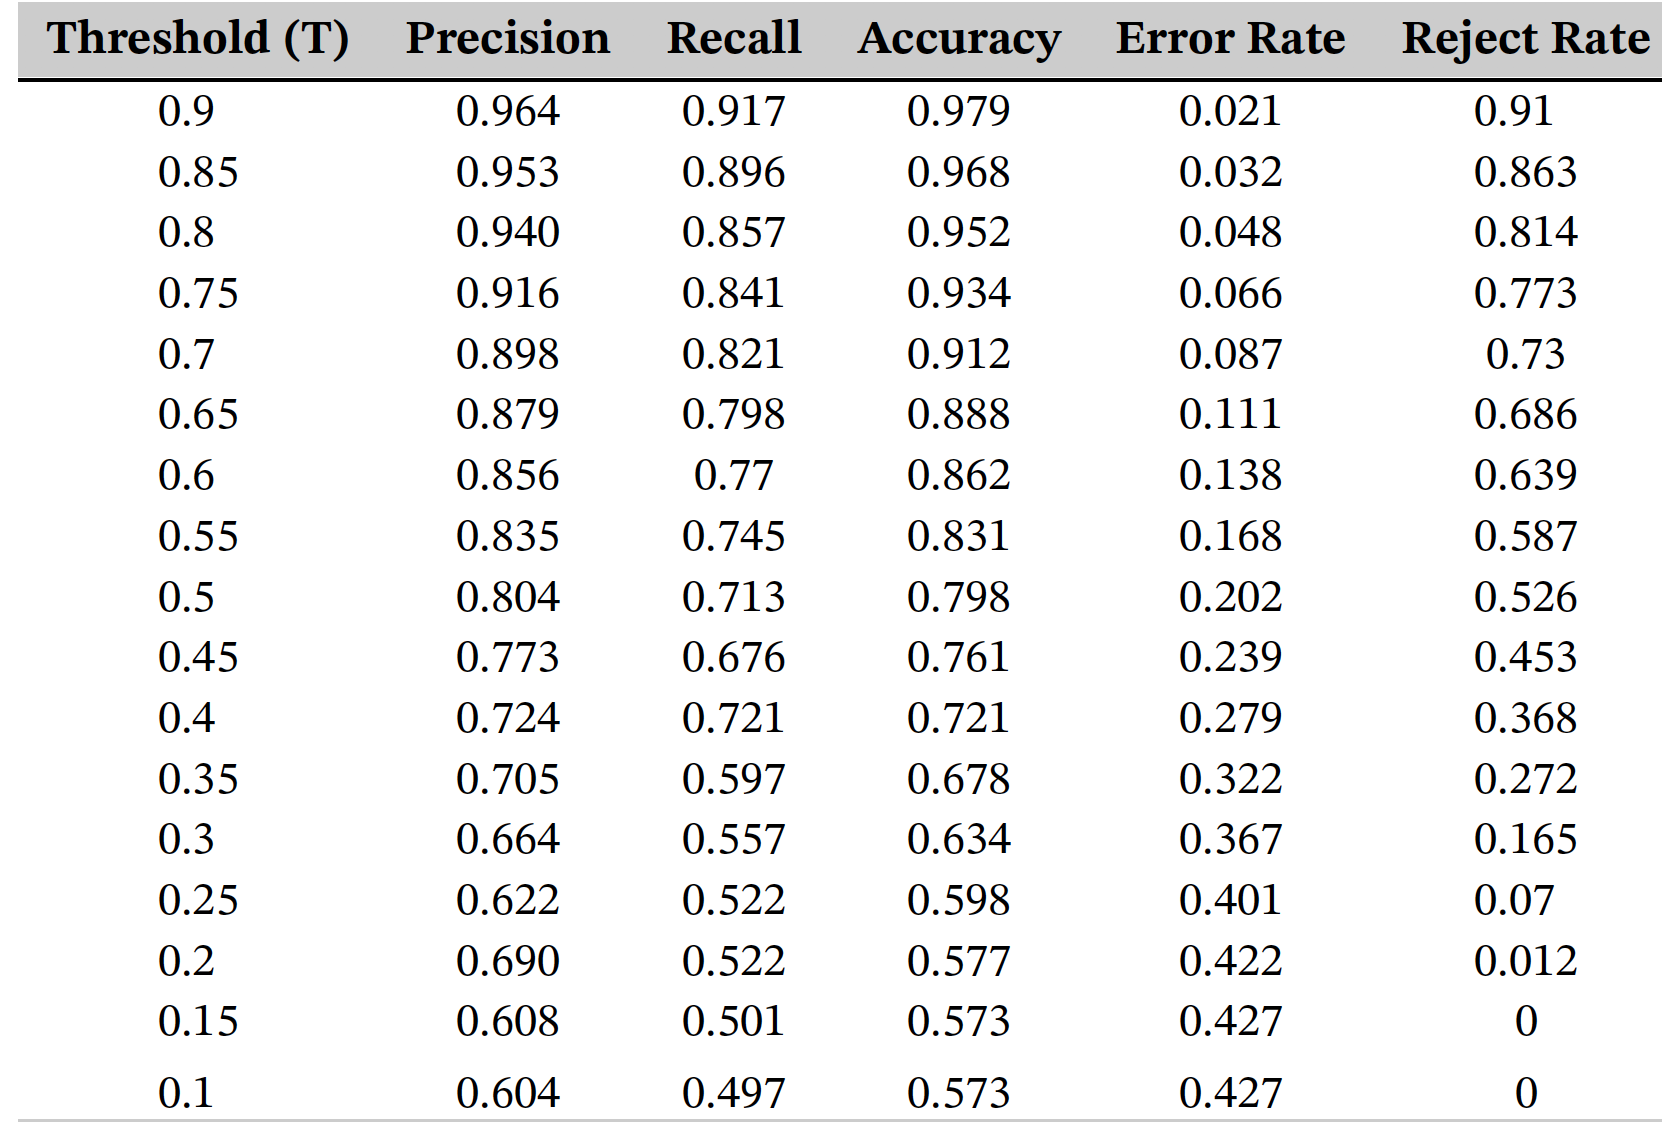
\includegraphics[width=90mm]{reject_acc.png}
    \caption{Model Metrics}
    \label{reject_acc}
\end{figure}

\begin{center}
\subsection{Convolutional Neural Networks for Sentence Classification}
\end{center}


Here we find a similar set up where \cite{kim2014convolutional} also uses 1D CNN with pre-trained word vectors. The author experimented with different variations where he froze the embeddings and used transfer learning to fine tune the embeddings. Both resulted in great accuracies, which suggests that pre-trained models can be used as universal feature extraction methods.

\begin{figure}[ht!]
\center
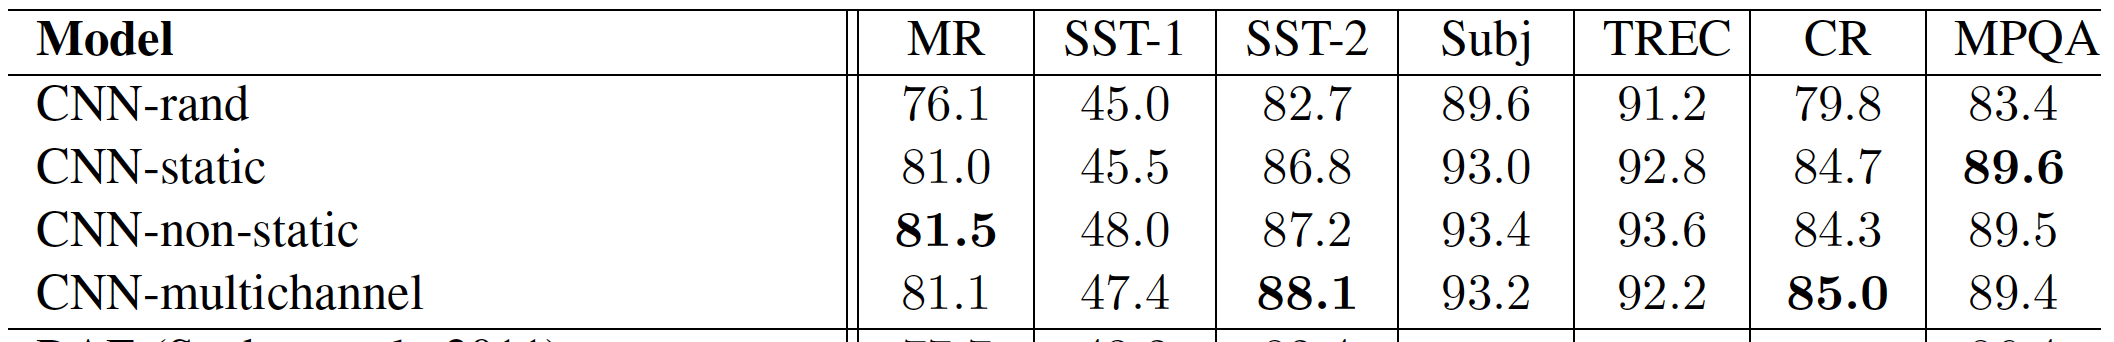
\includegraphics[width=130mm]{cnn_results.png}
    \caption{CNN Results}
    \label{cnn_results}
\end{figure}

As you can see from Figure \ref{cnn_results},  the CNN models surpassed state of the art on 4 out of 7 tasks, but which did not include any multiclass classifications. In figure \ref{cnn_arch}, we see the architecture of the CNN. 


\begin{figure}[ht!]
\center
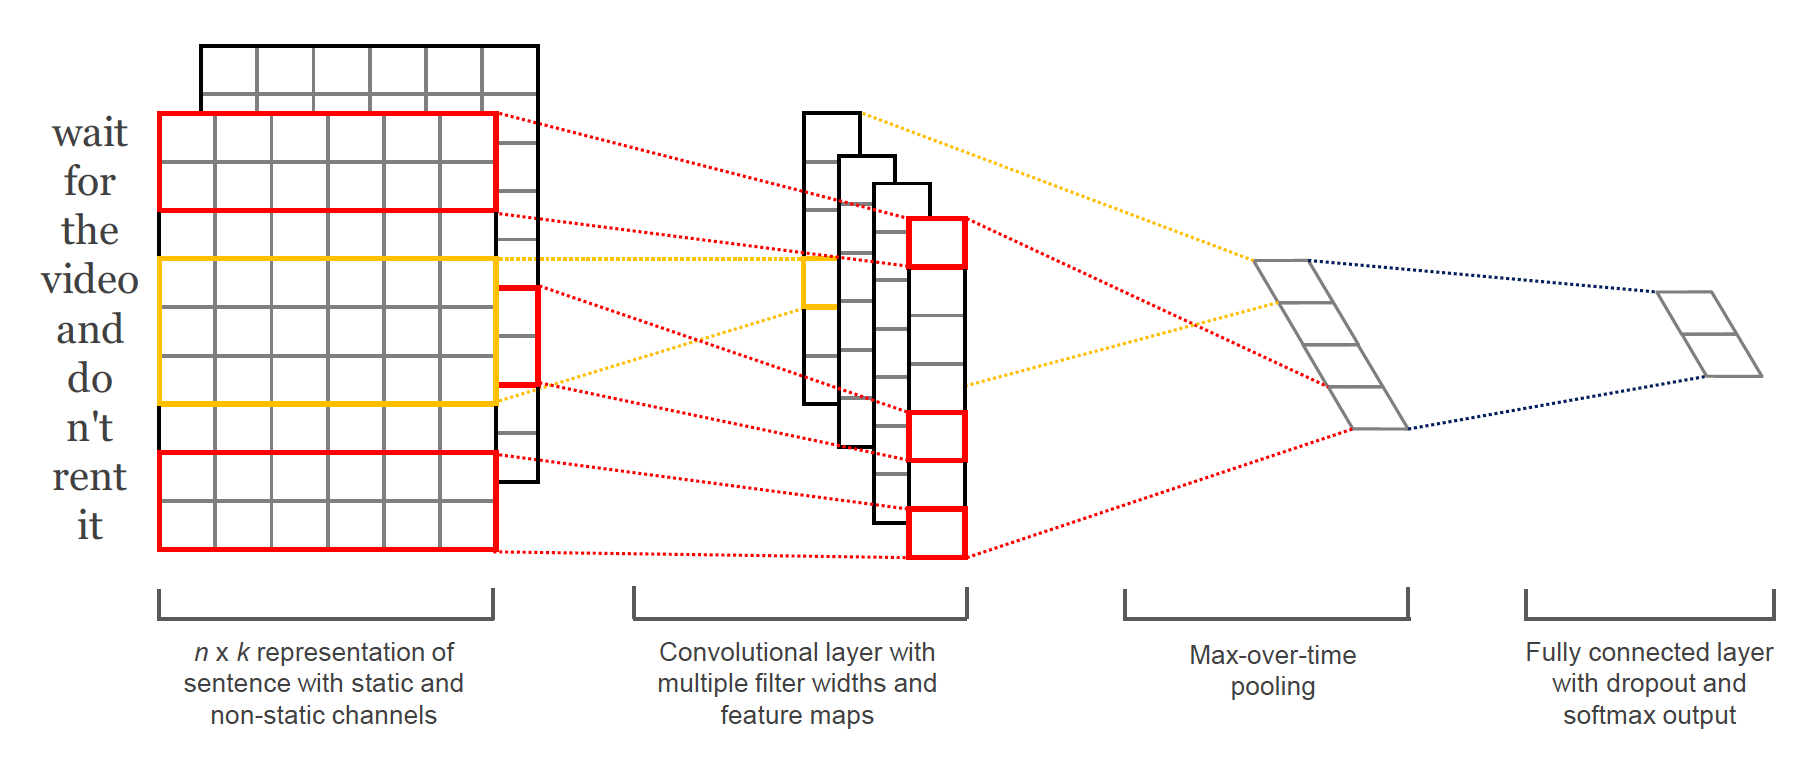
\includegraphics[width=130mm]{cnn_arch.png}
    \caption{CNN Architecture}
    \label{cnn_arch}
\end{figure}



\newpage
\section*{
\begin{center}
CHAPTER 3
\end{center}
\newline 
\begin{center}
STATISTICAL BACKGROUND AND METHODOLOGY
\end{center}}

\setcounter{subsection}{0}
\addtocounter{section}{1}

\begin{center}
\subsection{Preprocessing}
\end{center}


The processing steps generally include tokenization, normalization, and annotation. Tokenization is identifying and extracting terms. This can be as simple as using spaces to identify words in the English language but becomes more complex in other languages such as Mandarin. Normalization is stemming words such as transforming "running", "ran", "run" to "run" since they all convey the same meaning. Finally, we can annotate words which means differentiating between identical words that have different meaning depending on context. For example, fly can be a verb or a noun depending on the context. 

Removing stop words is an important process. Stop words are highly frequently used words that do not convey much meaning such as 'the', 'in', etc. There are many collections of stop words that can be downloaded for different languages. Here we plan to use Zipf's Law to identify stop words that are native to websites. For example, "contact" may be a stop word on domains because "Contact Us" is potentially very common on most websites. Traditional list of stop words will not have this insight.

Normalization increases recall and reduces precision but the opposite is true for annotation \cite{Turney:2010:FMV:1861751.1861756}. If we have a small corpus, the best option may be to normalize the text, to increase recall.

\begin{center}
\subsection{Zipf's Law}
\end{center}

While many scientific measurements may center at a typical point such as baby weights or human heights, some measures can vary by orders of magnitude such as wealth distribution. These measurements tend to be highly right-skewed. For example, the number of web hits during a single day is also right skewed meaning a small number of domains get a lot of hits while a lot of sites only get visited a few times. 

\begin{figure}[ht!]%
\centering
    \subfloat[Histogram]{{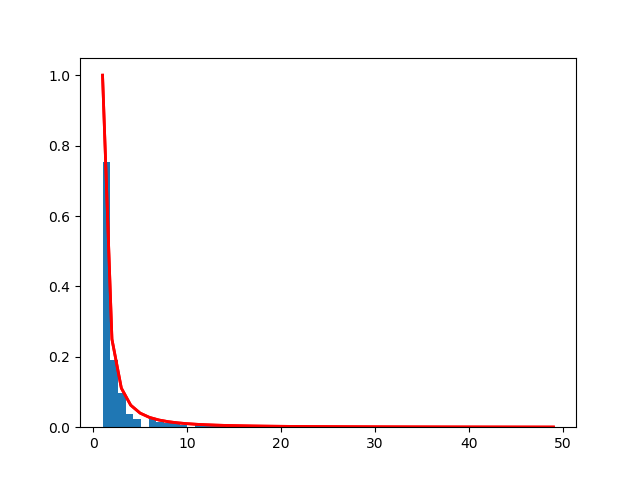
\includegraphics[width=9cm]{zipf.png} }}%
    \subfloat[Log Log Scale]{{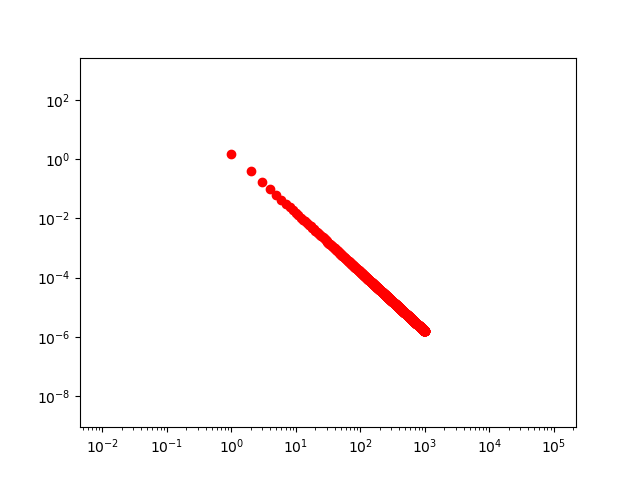
\includegraphics[width=9cm]{logscale.png} }}%
    \caption{Samples from a Zipf Distribution}%
    \label{fig:example}%
\end{figure}

From Figure 1(a), we can see the skewnedness of data coming from a Zipf Distribution. This closely mirrors the frequency of word usages where small percentage of words has almost all of the frequency distribution. The 80-20 rule is also another instance of this phenomena. 

Figure 1(b) highlights an interesting pattern. When we plot the data in a log-log scale, we see a straight line. This can be interpreted as follows. Let $p(x)dx$ be the proportion of observations between $x$ and $x + dx$. Furthermore, if we assume a straight line of the form $lnp(x) = -\alpha lnx+c$, then exponentiating both sides results in 

\begin{equation}
    p(x) = Cx^{-\alpha},\quad  where \quad C = e^c
\end{equation}

In general, cumulative distribution functions that follows Equation (1) are said to follow a Power Law, as well as  Zipf's Law, or Pareto Distribution \cite{newman2005power}. One can visualize this distribution by plotting a histogram. While finding the ideal binning width can be tricky, one can use the below equation, which represents the expected number of samples falling between $x_{min}\alpha^{k-l}$ and $x_{min}\alpha^k$ for the $k^{th}$ bin.


\begin{equation}
    \int_{x_{k-1}}^{x_k} p(x) dx = C  \int_{x_{k-1}}^{x_k} x^{-\alpha} dx = C \frac{{\alpha^{\alpha -1} - 1}}{{\alpha - 1}}(x_{min}\alpha^k)^{-\alpha + 1}
\end{equation}

Instead of plotting a histogram to verify if a sample follows a Zipf Distibution, we can plot the Complementary Cumulative Distribution Function (CCDF) defined as $\bar{F_X(x)} = P(X > x) = \int_x^\infty p_X(t) dt$ . Below is the equation pertaining to Zipf's Law.

\begin{equation}
    P(x) = \int_{x}^{\infty} p(x') dx' = C\int_{x}^{\infty} x'^{-\alpha} dx' = \frac{C}{\alpha - 1}x^{-(\alpha-1)}
\end{equation}

Notice that equation (3) also follows a power law but with exponent $\alpha - 1$. This means that if we were to plot in a logarithmic scales, then we would see a line again but with a shallower slope. Additionally, $\alpha$ can be estimated by fitting a linear regression but empirically the equation below works better (4) with an estimated expected error, $\sigma$ given by (5).


\begin{equation}
    \alpha = 1 + n\bigg[ \sum_{i=1}^{n} ln \frac{x_i}{x_{min}}\bigg]^{-1}
\end{equation}


\begin{equation}
    \sigma = \sqrt{n}\bigg[ \sum_{i=1}^{n} ln \frac{x_i}{x_{min}}\bigg]^{-1} = \frac{\alpha - 1}{\sqrt{n}}
\end{equation}

The constant C in equation (1) can be derived by normalizing the integral to equal 1. 

\begin{equation}
    1 = \int_{x_{min}}^{\infty} p(x) dx = C\int_{x_{min}}^{\infty} x^{-\alpha} dx = \frac{C}{1 - \alpha} \bigg[ x^{- \alpha + 1} \bigg ]_{x_{min}}^{\infty}
    \implies C = (\alpha - 1)x^{\alpha-1}_{min}
\end{equation}

Finally, equation (1) and (6) gives a normalized equation for the Power Law: 

\begin{equation}
    p(x) = \frac{\alpha - 1}{x_{min}}\bigg(\frac{x}{x_{min}}\bigg)^{-\alpha}
\end{equation}

Furthermore, \cite{LANDAUER200243} estimates that 80\% of the meaning of English text comes from word choice and the remaining 20\% comes from word order. Assuming fraction of the words whose frequency exceeds $x$ is given by the quantity $P(x)$. The fraction of the total frequency in the set of those words are: 

\begin{equation}
    W(x) = \frac{\int_{x}^{\infty} x'p(x') dx'}{\int_{x_{min}}^{\infty} x'p(x') dx'} = \bigg(\frac{x}{x_{min}}\bigg)^{-\alpha+2}
\end{equation}

\begin{center}
\subsection{Vector Space Models of Semantics}
\end{center}

\cite{Turney:2010:FMV:1861751.1861756} describes Vector Space Models (VSM) as a system that creates embeddings for documents (phrases/words) which maps them in a vector space such that semantically similar documents are close in distance. This automatic feature extraction method reduces the dependency of laborious semantic approaches such as lexicons and ontologies. Additionally, elements in a VSM must be of a frequentist nature.

The statistical semantics hypothesis: statistical patterns of human word usage can be used to figure out what people mean. This general hypothesis underlies several more specific hypotheses, such as the bag of words hypothesis, the distributional hypothesis, the extended distributional hypothesis, and the latent relation hypothesis, discussed below.

The statistical semantics hypothesis states that statistical analysis of human language usage can be used to deduce meaning. Hypotheses such as bag of words and distributional hypothesis fall under this more general hypothesis. The distributional hypothesis follows the idea that one can derive the meaning of a word by its context. 

Latent Meaning describes the use of Truncated Singular Value Decomposition, $\hat{X} = U_k \sum_k V_k^T$, which maps vector spaces into a lower dimension. This mathematical operation helps capture the latent (hidden) meaning in words and context. By forcing a dimensionality reduction from say k to r, where $k < r$, the restricted concurrence between words and contexts increases similarity. Similarity can be measured using cosine similarity described in Equation (10).

\begin{equation}
\textbf{x} = \big \langle x_1, x_2, ... , x_n \big \rangle \quad
\textbf{y} = \big \langle y_1, y_2, ... , y_n \big \rangle
\end{equation}

\begin{equation}
cos(\textbf{x}, \textbf{y}) = \frac{\sum_{i=1}^{n} x_i y_i}{\sqrt{\sum_{i=1}^{n} x_i^2 \sum_{i=1}^{n} y_i^2}} = \frac{\textbf{x}}{\|\textbf{x}\|}\frac{\textbf{y}}{\|\textbf{y}\|}
\end{equation}

There is an assumed notion of similarity between documents when building machine leaning tasks to classify or cluster them.

\begin{center}
\subsection{Word Vector Representations}
\end{center}

Word vectors are a numerical representation of words where if mapped on to a vector space, then semantically similar words will be close. These vectors are dense and fixed length, usually 100 to 1,000 dimensions, which makes great inputs for machine learning tasks. Word2vec, which follows this framework, was famously introduced by Tomas Mikolov at Google.
 
 
\subsubsection{Skip-gram}

\cite{NIPS2013_5021} uses the idea that the context of the words defines the word. This uses neural networks to predict a word given a sequence of words. This surprisingly has linear relationships. For example, the operation vec("Madrid") - vec("Spain") + vec("France") is closest to the vec("Paris") than any other word vector representation. It tries to maximize the average log probability $\frac{1}{T}\sum\sum log p(w_{t+j} | w_t)$ where $p(w_0 | w_I) = \frac{exp(v_{w0}^T v_{wI})}{\sum exp(v_{w}^T v_{wI}) }$ where $v$ are the input and output vector representations of $w$.

\subsubsection{Hierarchical Softmax}

The issue of the Skip-gram is that it computationally expensive so Hierarchical Softmax is good alternative for calculating conditional probabilities. Here, they use a tree structure called Huffman tree to efficiently find common words. This tries to approximately maximize the average log probability \cite{NIPS2013_5021}. 

\begin{equation}
  p(w|w_1) = \Pi \sigma (\llbracket n(w,j+1) = ch(n(w,j))  \rrbracket  * v_n ^ T v_{wI})
\end{equation}


\subsubsection{Noise Contrastive Estimation (NCE)}

The intuition is that a good model should be able to differentiate real words from noise using a classifier such as logistic regression. This also tends to approximately maximize the average log probability but is mainly concerned with learning quality vector representations. Here $P_n(w)$ is a noise distribution where they found that a uniform distribution raised to the 0.75 power outperforms usual uniform distribution \cite{NIPS2013_5021}.

\begin{equation}
    log \sigma(v_{w0}^T v_{wI}) + \sum \EX_{wi} \sim P_n(w)[log\sigma(-v_{wi}^T v_{wI})]
\end{equation}

\begin{center}
\subsection{Paragraph or Document Vector Representations}
\end{center}

Extending the idea of word vectors, document vector representations attempts to generate a numerical representation of documents. Here we discuss frameworks that while conceptually simple, surprisingly, produce performing feature extraction methods.  

\subsubsection{Bag of Words}

Bag of words is simple approach for representing documents in a fixed-length vector. It has the following structure: $\{word_1: frequency_1, word_2: frequency_2, ... , word_n: frequency_n \}$. While it is easy to train, it has multiple disadvantages. This does not capture any semantics and quite sparse.

\subsubsection{TF-IDF} 
\label{TF-IDF}
Term frequency-inverse document frequency is a transformation method of text data to a numeric matrix that reflects the importance of a term to a website in the corpus. 

Let $t$ = a term (word), $d$ = a document (website), and $D$ = the corpus (the collection of websites). Let TF($t$, $f$) be a function that counts the number of times a term appears in a website (Term Frequency) and DF($t$, $D$) be a function that counts the number of websites that contains the term $t$. Then TF-IDF is the product of TF and IDF, such that

\begin{equation*}\label{eq:pareto mle2}
\begin{multlined}
IDF(t,D) = log \frac{|D|}{DF(t, d) + 1}
\end{multlined}
\end{equation*}

\begin{equation*}\label{eq:pareto mle2}
\begin{multlined}
TFIDF(t, d, D) = TF(t, d) \cdot DF(t, D)
\end{multlined}
\end{equation*}

where $|D|$ is the total number of documents in the corpus. Notice that a smoothing term is applied to avoid dividing by zero. TF-IDF provides a way to emphasize important words and give less weight to terms that appear in many websites which probably will not have much importance like common words such as "the".

\begin{center}
\subsection{Advance Paragraph or Document Vector Representations}
\end{center}

In this section, we explore state of the art feature extraction methods. These VSMs use techniques that go beyond a frequentist approach but use deep learning frameworks to create semantically dense document representations that are highly performing. 

\subsubsection{Paragraph Vectors}

Very similar to the skip-gram approach for word vectors. The intuition is that this model provided quality vector representations for words given a supervised task of predicting the next word in the sequence. For paragraph vectors they attempt to do the same but just adding a paragraph id represented as a matrix while jointly trying to predict words in that paragraph \cite{Le:2014:DRS:3044805.3045025}. 

\begin{figure}[ht!]
\center
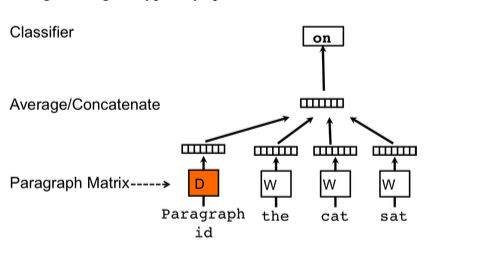
\includegraphics[width=90mm]{paragraph.png}
    \caption{Paragraph Vector}
    \label{paragraph vector}
\end{figure}

\subsubsection{Concatenated Power Mean Word Embeddings}

The idea is to generalize averaging word vectors to represent documents. The problem with earlier attempts is that naively averaging word vectors causes information loss about the ordering of the words. This new method attempts to concatenate different averaged word vectors to capture both the ordering a different signals such a semantic information. The power means generalize this function \cite{DBLP:journals/corr/abs-1803-01400}. 

Power Means: 
\begin{equation}
    (\frac{x_1^p + ... + x_n^p}{n})^{1/p}
\end{equation}

Sentence Vector:
\begin{equation}
    s^{(i)} = H_{p1}(W^{(i)}) \oplus ...  \oplus H_{pk}(W^{(i)})
\end{equation}

Where $H_p(W)$ is a vector whose d components are the power means of the sequences $(w_{1i} , ... , w_{ni}) $ and $\oplus$ stands for concatenation of $p_1 , ... , p_k$, which are K different power mean values.

\subsubsection{GloVe - Global Vectors for Word Representation}
GloVe vectors are similar to Word2Vec vectors but generally perform better. While Word2Vec mainly takes into account the local neighborhood of a word, GloVe vectors consider global context. That means they look at the whole document when generating a word vector instead of just the surrounding words.

Just as Word2Vec, GloVe is an unsupervised learning algorithm that maps words into vector space where distances between words are related to their similarity. It does so by counting how often two words co-occur and then finding the global optimum of some probability function.

The objective is to choose the word vectors in a way so that their dot product equals the logarithm of the words' probability of co-occurrence.

We mapped the GloVe vectors generated by a pretrained model into 2D space using T-SNE and PCA. 
It can be seen that the embbedings for the websites have a lot of potential for discriminating between categories. Some of the clusters are kind of spread out but that is probably owed to the dimensionality reduction applied before.



\begin{center}
\subsection{Classification}
\end{center}

Classification algorithms are a type supervised learning. Generally, the input is data that is labeled into categories. Then using this ground truth, the model is trained to fit the data to be used for predicting labels for new observations. In our study, we use Multinomial Logistic Regression (MLOGIT) and one dimensional Convolutional Neural Network (CNN), which we will discuss in future chapters. 

\subsubsection{Logistc Regression}
Logistic Regression is a supervised machine learning algorithm that used for classification.  Let signal $s = \textbf{w}^T\textbf{x}$ where $\textbf{x}$ are input data and $\textbf{w}$ is weight matrix then the logistic regression model (hypothesis) has the form \cite{Abu-Mostafa:2012:LD:2207825}:

\begin{equation}
    h(s) = \theta(s) = \frac{e^s}{1+e^s}, \quad \theta \in [0, 1]
\end{equation}




\begin{figure}[ht!]
\center
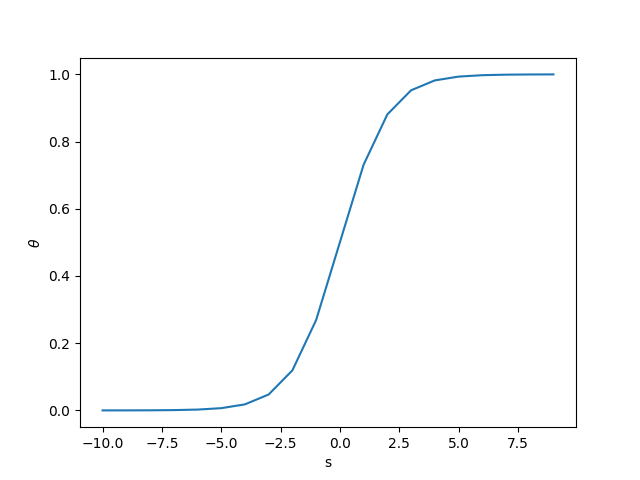
\includegraphics[width=90mm]{sigmoid.png}
    \caption{Sigmoid Plot}
    \label{sigmoid}
\end{figure}



You can see sigmoid plot in \ref{sigmoid}. Given a set of labels, $y \in \{+1, -1\}$, then the likelihood of mapping output $y$ from input $\textbf{x}$ is given by a targeting distribution $P(y|\textbf{x})$. If we believe this is capture by our hypothesis then we can define the likelihood as

\begin{equation}
\label{eq:1}
 P(y|\textbf{x}) =
    \begin{cases}
      h(\textbf{x}) & \text{for $y = +1$}\\
      1 - h(\textbf{x}) & \text{for $y = -1$}\\
      \end{cases}       
\end{equation}

Because $h(-x) = 1 - h(x)$, then Equation \ref{eq:1} becomes 

\begin{equation}
    \label{eq:2}
    P(y|x) = \theta(y\textbf{w}^T\textbf{x})
\end{equation}

Using maximum likelihood we can maximize the likelihood function defined as $ {\displaystyle \prod_{n=1}^N P(y_n | x_n)}$ or minimize $-\frac{1}{N}ln\Big({\displaystyle \prod_{n=1}^N P(y_n | x_n)}\Big) = \frac{1}{N}{\displaystyle \sum_{n=1}^N} ln\Big(\frac{1}{P(y_n | x_n)}\Big) = \frac{1}{N}{\displaystyle \sum_{n=1}^N} ln\Big(\frac{1}{\theta(y\textbf{w}^T\textbf{x})}\Big) $

\begin{equation}
    \label{eq:3}
    E_{in}(w) = \frac{1}{N} \sum_{n=1}^N ln\big(1 + e^{ -y_n w^T x_n } \big)
\end{equation}

Computing the gradient, we get

\begin{equation}
    \label{eq:3}
    \nabla E_{in}(w(t)) = - \frac{1}{N} \sum_{n=1}^N \frac{y_n x_n}{1 + e^{ y_n w(t)^T x_n } }
\end{equation}


The pseducode for updating weights where $a$ is the learning rate
\begin{verbatim}
    set initial weights at t=0
    for t=0 to max_iteration
        calculate gradient, Ein (equation 19)
        update weights w(t+1) = w(t) - a*Ein
\end{verbatim}


For a Multinomial Logisitc Regression model where there is more than two classes. Then we use a softmax function. Let $s = f(x_i, W)$, then we have a softmax function defined as 

\begin{equation}
P(Y=k|X=x_i) = \frac{e^s_k}{\sum_j e^s_j}
\end{equation}

Where cross-entropy loss that has the form:

\begin{equation}
L_i = -\log\left(\frac{e^{f_{y_i}}}{ \sum_j e^{f_j} }\right) \hspace{0.5in} \text{or equivalently} \hspace{0.5in} L_i = -f_{y_i} + \log\sum_j e^{f_j}
\end{equation}



\subsubsection{Convolutional Neural Network (CNN)}


CNNs have traditionally been used for image classification. As supposed to fully connected layers, which may overfit data, CNNs are useful when there is a spatial correlation that can be found in pixels. CNNs are composed of neurons with weights and biases that get updated at each iteration to minimize some loss function. One of the main differences between CNNs and neural networks (NN), is that NN's have vectors as inputs, whereas the input is a multi-channeled image for CNN's. Below is a visualization of convolution.

\begin{figure}[ht!]%
\centering
    \subfloat[Step 1]{{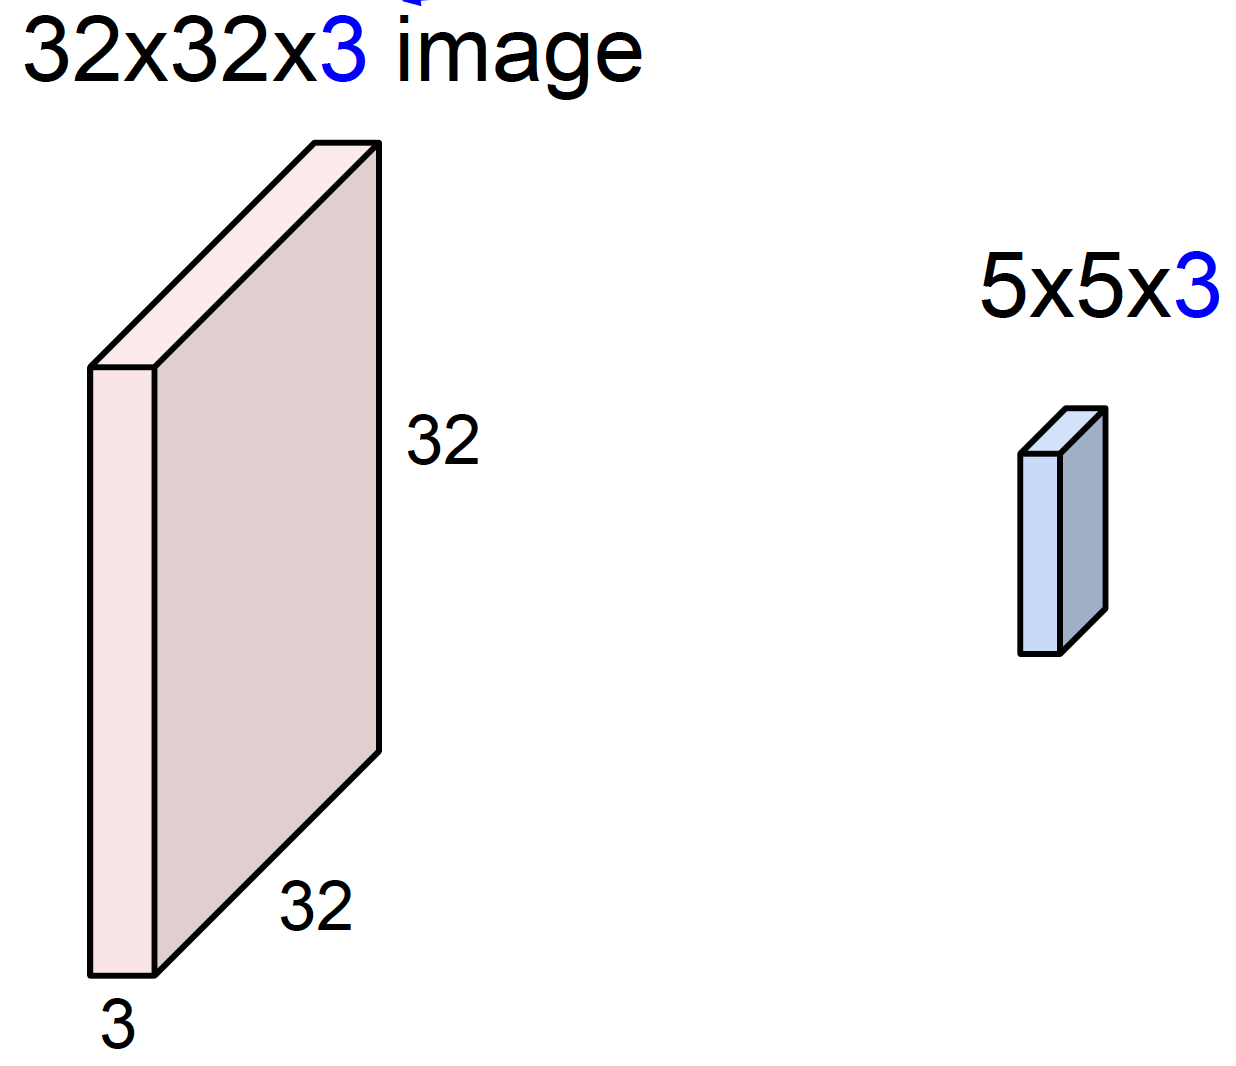
\includegraphics[width=9cm]{step1_cnn.png} }}%
    \subfloat[Step 2]{{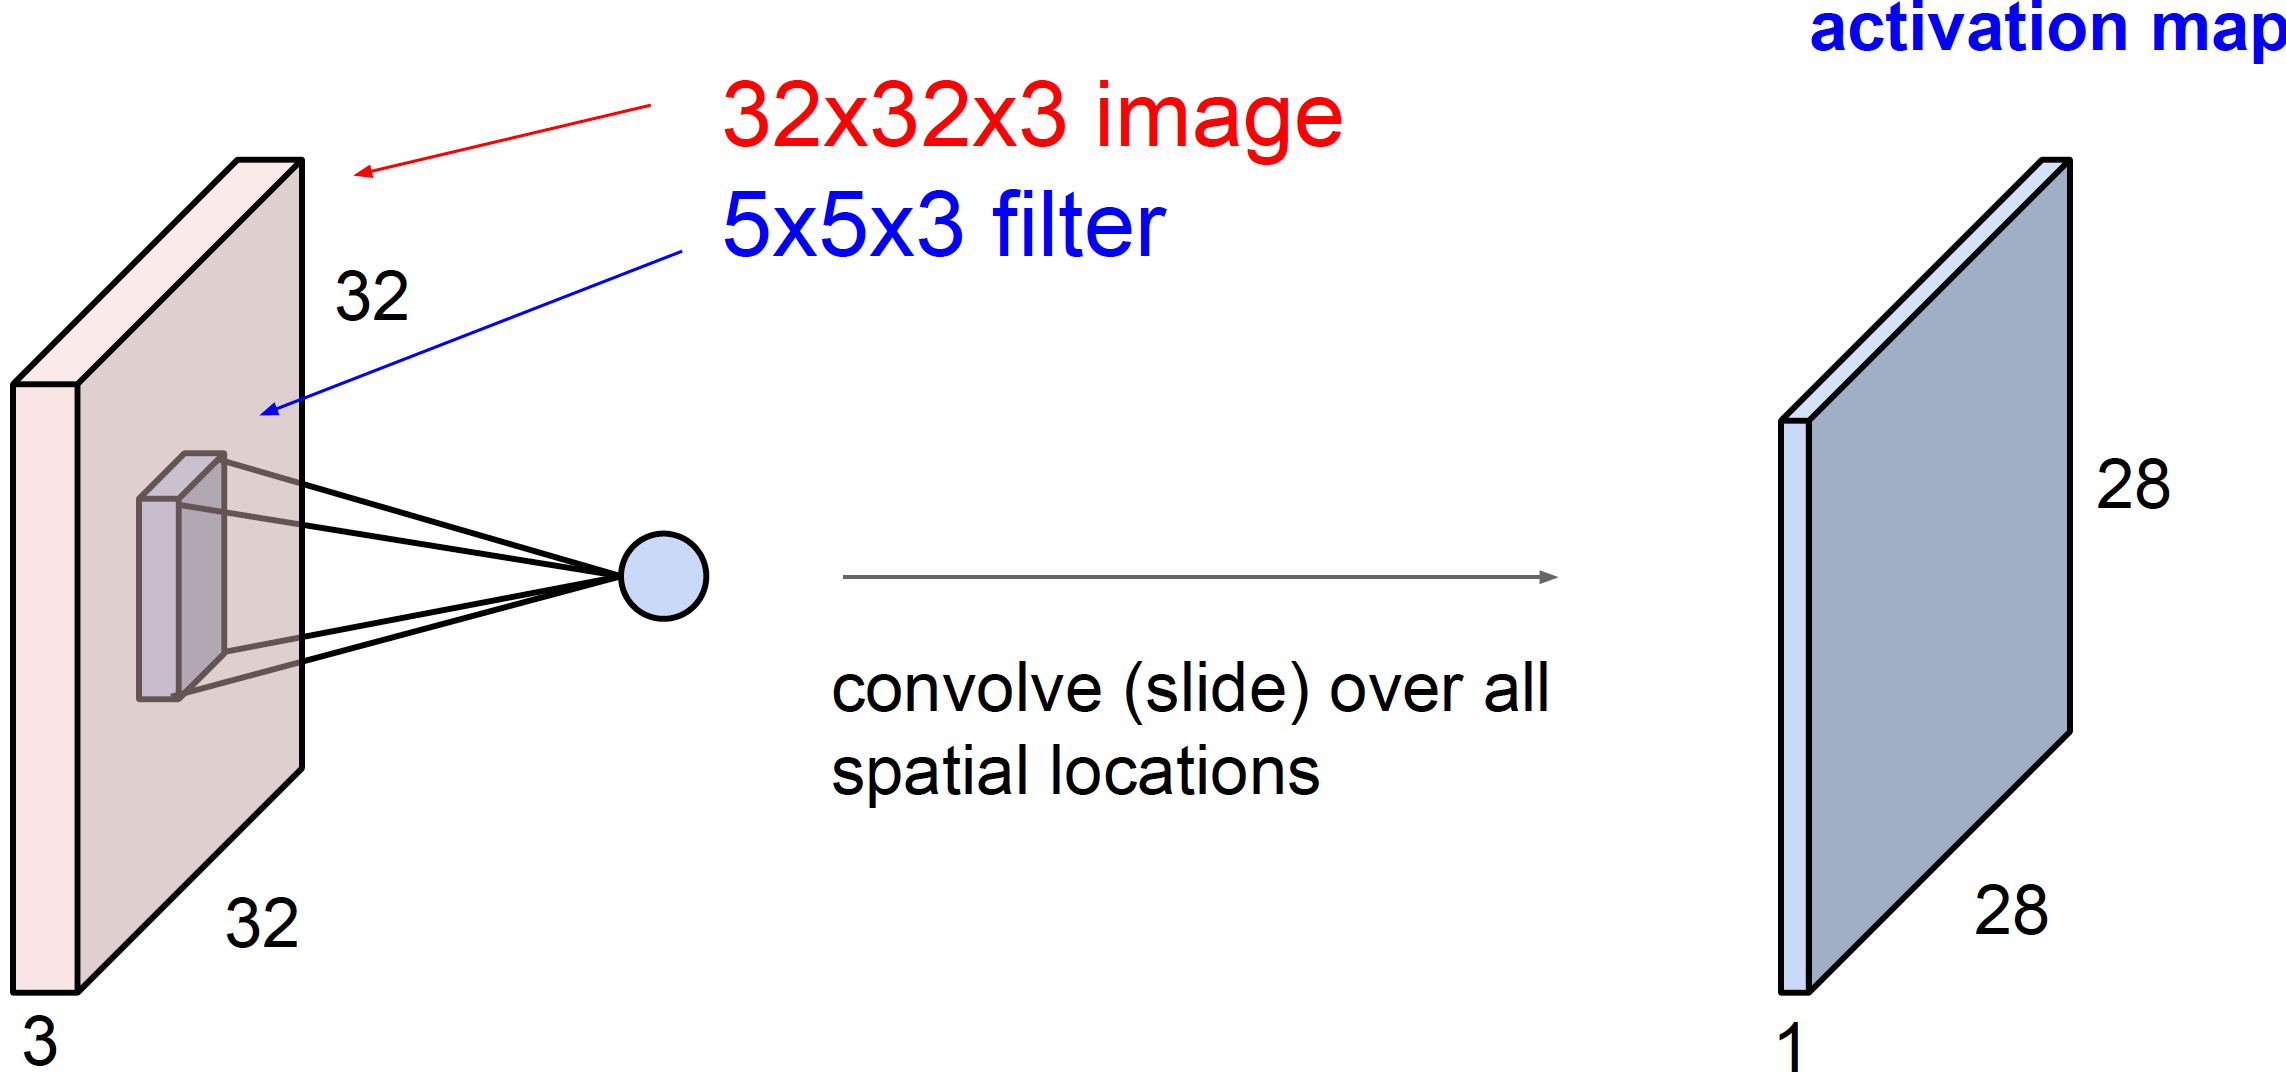
\includegraphics[width=9cm]{step2_cnn.png} }}%
    \caption{Convolution \cite{cs231}}%
    \label{fig:cnn}%
\end{figure}




CNNs have different types of layers \cite{chollet2015keras}. The Embedding layer can be seen as a dictionary that maps integers words (or indices) to dense vectors. A 1D Convolution Layer implements a convolution kernel which convolves the input layer over a one dimensional spatial dimension producing a tensor. Also, Dropout  Layers apply dropout to the input layer, which randomly sets some neuron weights to zero, which helps with overfitting. Furthermore, a Dense Layers is a regular densely-connected neural network layer. Operations such as Max pooling is also common operations that eliminates redundant information. Global max pooling is the same as max pooling layer but with pool size that equals to the size of the input. For example, if the input of the max pooling layer is 0,1,2,2,5,1,2 then the global max pooling outputs 5. In our case, we use a one dimensional version of CNN because sentences have an one dimensional spatial correlation. 





\newpage
\section*{
\begin{center}
CHAPTER 4 
\end{center}
\newline 
\begin{center}
AUTOMATIC TEXT CLASSIFICATION BASED ON ZIPF’S LAW
\end{center}}

\setcounter{subsection}{0}
\addtocounter{section}{1}

\cite{Yatsko:2015:ATC:2813730.2813744} proposes to use Zipf's Law for segmentation to automatically classify websites. His segmentation rule is as follows:

\begin{quote}
The method of zonal processing involves dividing each text into three zones: J0, J1 and J2. The J0 zone includes stop words. Since it has the smallest number of elements with the highest frequency, it can be called a zone of information concentration. The J1 zone consists of notional words that reflect the content of the text. The J2 zone contains rarely used words, abbreviations, and neologisms coined by the author. It is the area of the largest information dissemination, as it contains the largest number of elements with the lowest frequency.
\end{quote}

\cite{Yatsko:2015:ATC:2813730.2813744} uses zone J0 as inputs for a classification model. He calculates the deviation between the theoretical word frequencies in $J_0$ and the empirical ones as a signal for classification. We intend to explore using J1 as a pre-processing step instead. If words in $J_1$ reflects the content of the text, then would like to use those words as input for the machine learning pipeline in Figure \ref{pipeline}.

\begin{figure}[ht!]
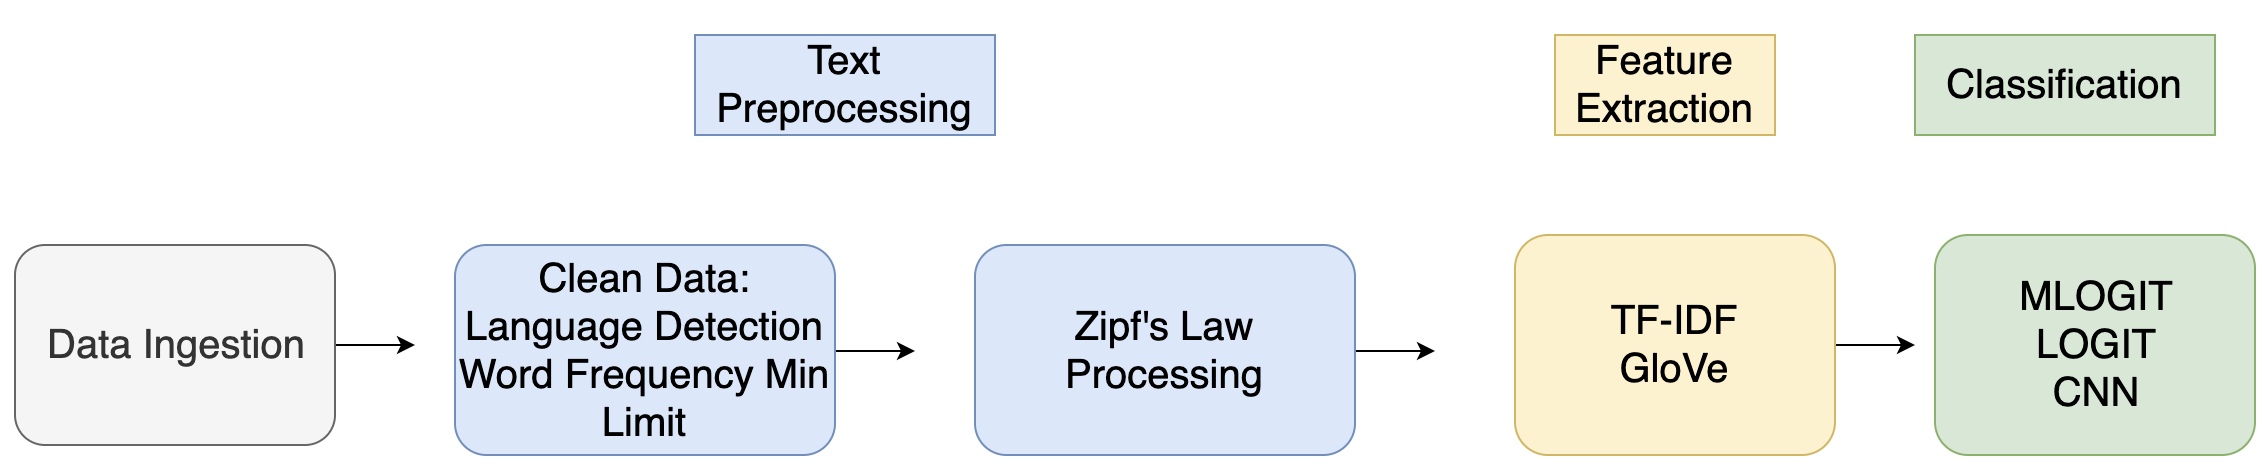
\includegraphics[width=160mm]{workflow.png}
    \caption{Workflow}
    \label{pipeline}
\end{figure}

\begin{center}
\subsection{Motivation}
\end{center}

In this previous work \cite{previous}, we investigated three feature extraction methods and three clustering algorithms for their effectiveness in creating clusters with low within cluster sum of square errors (WCSSE). The three clustering algorithms investigated include two well-known clustering techniques, K-means and Bisecting K-means,and one newly developed variant called SphericalK-Means. The three feature extraction methods investigated include two well-known methods, countvectorization and term-frequency inverse document-frequency (TF-IDF), and one newer method called Hashing Term-Frequency. In order to generalize our results for multiple languages, text was collected from websites in three languages: English, Spanish,and Korean. Using a 2-Factor ANOVA with a block on language, we assessed which feature extraction method, clustering algorithm, and feature extraction-clustering algorithm combination resulted in clusterswith the lowest WCSSE. Our results suggest that TF-IDF resulted in forming clusters with the lowest WCSSE regardless of paired clustering algorithm.

\subsubsection{Two-Factor ANOVA with Blocking}

\textbf{Objective:} Determine which feature extraction method and clustering algorithm pair forms clusters with the smallest within cluster sum of square errors blocking for language effect.
\vspace{5mm}  

\textbf{Model:}
\begin{equation}
Y_{ijk} = \mu + \alpha_{i} + \beta_{j} + (\alpha\beta)_{ij} + \delta_{k} + \epsilon_{ijk}
\end{equation}


\textbf{Response Variable $Y$ :} Within Cluster Sum of Square Errors (WCSSE). 
\vspace{3mm}  

\textbf{Treatment Effect $\alpha$ :} Feature Extraction Algorithm for $i = 1,2,3 $ where $\alpha_{1}$ is CountVectorizer, $\alpha_{2}$ is TF-IDF, and $\alpha_{3}$ is Hashing TF-IDF.
\vspace{3mm}  

\textbf{Treatment Effect $\beta$ :} Clustering Algorithm for $j = 1,2,3$ where
$\beta_{1}$ is K-Means,
$\beta_{2}$ is Bisecting K-Means, and
$\beta_{3}$ is Spherical K-Means.
\vspace{3mm}  

\textbf{Block Effect $\delta$ :} Clustering Algorithm, for $k = 1,2,3$ where
$\delta{1}$ is English,
$\delta{2}$ is Spanish, and
$\delta{3}$ is Korean.
\vspace{3mm}  

\textbf{Interaction Effect:} 
$\alpha\beta$ : Feature Extraction Algorithm *  Clustering Algorithm for all $i$ and $j$.


\begin{figure}[ht!]
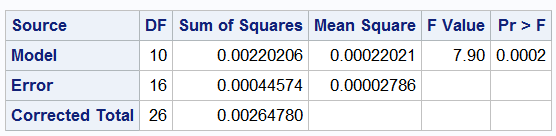
\includegraphics[width=75mm]{anova1.PNG}
    \caption{Overall Model}
\end{figure}


\begin{figure}[ht!]
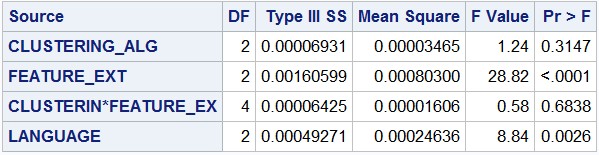
\includegraphics[width=75mm]{anova2.PNG}
    \caption{Factors}
\end{figure}


From the ANOVA table, we see that the overall model is significant at the 0.05 significance level. However, Figure 5 shows that the Feature extraction method and block effect are the only actual statistically significant affect on WCSSE. 

\begin{figure*}[h]
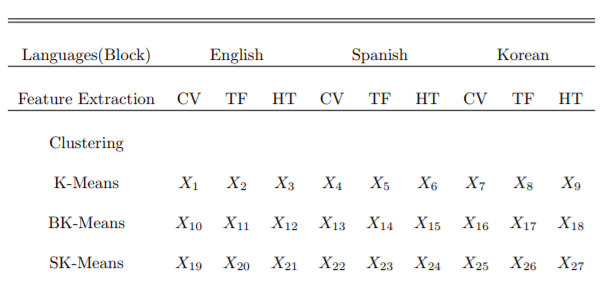
\includegraphics[]{table.PNG}
\caption{Two Factor ANOVA with Blocking}
\end{figure*}

This study highlights that feature extraction methods are vital for machine learning task related to website modeling. Hence, we continued researching more advance VSMs as discussed in previous chapter.

\begin{center}
\subsection{Zipf's Law}
\end{center}

We also used Zipf's Law to do exploratory data analysis. A rigorous analysis of Zipf's law is made using an index for the sequence of observed values of the variables in a Zipf-type relationship. Three important properties relating rank, count, and frequency are identified. For example, Zipf's law states that given some corpus of natural language utterances, the frequency of any word is inversely proportional to its rank in the frequency table. Thus the most frequent word will occur approximately twice as often as the second most frequent word, three times as often as the third most frequent word, etc. The rank-frequency distribution is an inverse relation. It follows a probability density function:

\begin{equation}
P(x) = \frac{x^{-\rho + 1}}{\zeta(\rho + 1)}
\end{equation}

Where $\rho$ is positive parameter and $\zeta(z)$ is the Rieman Zeta Function [2]

We can appreciate Zipf's law reflected in our data by plotting the data on a log-log graph with the axes being log (rank order) and log (frequency). The data follows Zipf's law to the extent that the plot is linear.

\begin{figure}[ht!]
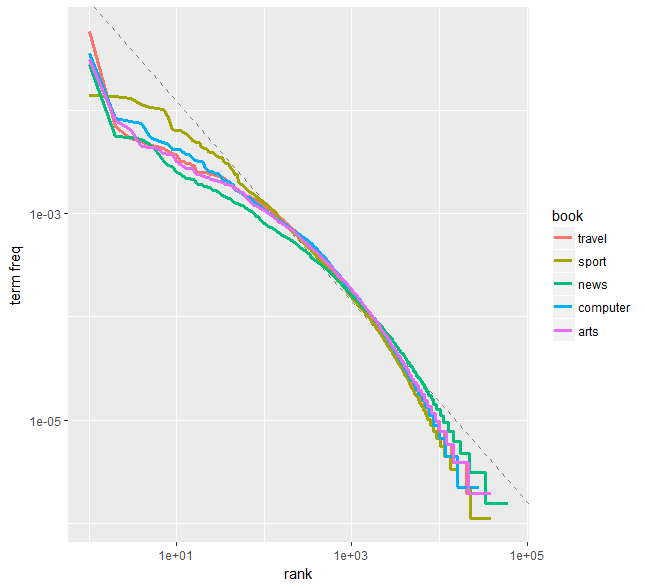
\includegraphics[width=100.49mm]{zipfs_law.png}
    \caption{Zipf's Law}
\end{figure}

Comparing the distribution to a simple regression line in Figure 7, we see that the tails of the distribution deviate suggesting our distribution doesn’t follow Zipf’s law exactly, but it is close enough to state that the law approximately holds within our corpus of websites. In fact from fitting a regression model, we get an R-squared of 0.9473 with significant intercept and slope. TF-IDF transformation is very much motivated by Zipf's law, in that the log term is there because of Zipf's law. 


\begin{figure}[ht!]
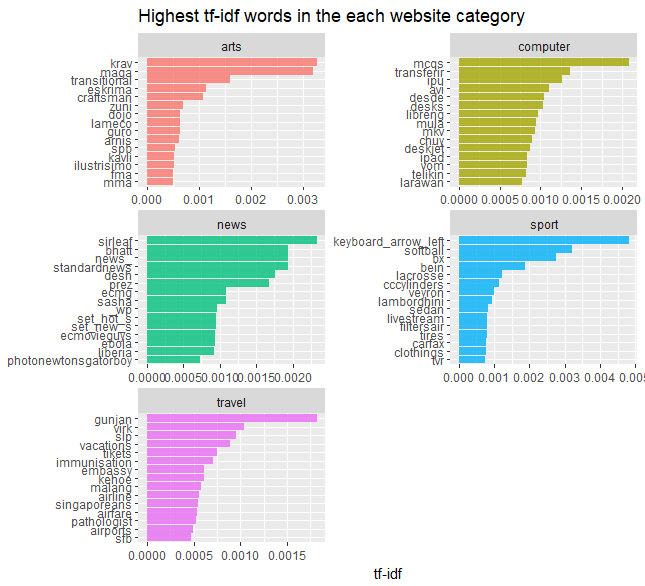
\includegraphics[width=100mm]{tfidf.png}
    \caption{TF-IDF Per Category}
\end{figure}

As we can see from Figure 8, we see relevant words that have a high TF-IDF score for their respective category. For example, arts has craftsman, computer has ipad, news has standard news, sport has softball, and travel has vacations. The other words that are less relevant were probably given a high score because they were more rare so the inverse log score would have given a bigger score. This means that these particular words standout and give us a more unique look at each category. For example, the arts category has the word eskrima which is a martial art of the Phillipines. This means that when we gathered arts websites it got not only arts websites relating to craftsmanship but also martial arts websites. This may lead to some classification errors.

\begin{center}
\subsection{Multinomial Logistic Regression}
\end{center}

\subsubsection{TF-IDF and MLOGIT}
Multinomial Logistic Regression model was used as a base model for benchmarking due to its simplicity. Also MLOGITs usually still work well even when the amount of data available is not huge. For the feature extraction we first used the TF-IDF representation of the website texts. Our goal was to compare different feature extraction methods in order to find out which one performs the best.

We split the cleaned dataset into 70 \% training and 30 \% test. After that we used the \texttt{sklearn} \texttt{Pipeline} class to apply the three sequential transformations to the training data. The first step is the \texttt{CountVectorizer} which converts our website texts to a matrix of token counts. This count matrix will be  transformed to a normalized TF-IDF representation using the \texttt{sklearn} \texttt{TfidfTransformer}. The theory behind the general TF-IDF transformation is described in section \ref{TF-IDF}. Since this was used a base model, we used all the default parameters.

As it turns out, this very simple linear model actually yields very good results regarding accuracy. On the test data (which we split from the original dataset and has the size of 30 \% of the whole dataset) it reaches an accuracy of 90.5\% which is about twice as good as a classifier that would always guess "Sports". 


\subsubsection{GloVe vectors and MLOGIT}
For our next approach we wanted to test how much better or worse a more complex feature extraction method performs compared to TF-IDF.
The method we decided to use was GloVe vectors.
They were created using a pretrained model from the Python NLP library Spacy.

This model was trained on the dataset Common Crawl which is a large corpora that provides text scraped from websites.
Since we are working with website text classification this model seemed to fit our purpose very well. 

The worfklow was the following: After downloading the pretrained model, we load it into the Python script. We only use it for inference by inputting all of our text data and saving the resulting document vectors. These document vectors are then used to train a MLOGIT which performs the classification based on those vectors. The output of the MLOGIT is the label of the input text. Surprisingly, this more complex model performed a little worse than the TF-IDF approach. The accuracy across all classes was 89.5\%.

\begin{center}
\subsection{Convolutional Neural Network}
\end{center}


\subsubsection{Architecture}

The architecture is summarized in Figure 9. It is composed of an embedding layer that has pretrained glove model for the word vectors. We make sure to freeze them for training because we do not want to erase the learned weights. It is then followed by 1D convolution layers each followed by either a max pooling or a global max pooling layer. We then finish with two dense layers with a dropout layer between them. The final dense layer has dimension (None, 4) with a softmax activation function which tries to predict the probability of belonging in one of the four categories.


\begin{figure}[ht!]
\center
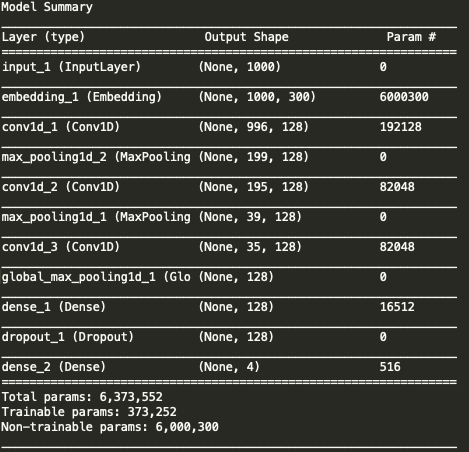
\includegraphics[width=90mm]{model_architecture.png}
    \caption{Model Architecture}
    \label{instances_classes}
\end{figure}




Initially, our model had an overfitting issue. For this attempt we did not do any hyperparameter tuning so it was not too suprising to see overfitting. This issue was also present for the loss metric. We tried different approaches such as using batch normalization and adding a dropout layer to reduce overfitting. Ultimately, the dropout layer gave the best result. After some hyperparameter tuning, we settled for a droput rate of 30\%.


\subsubsection{GloVe vectors and CNN}

The intuition was to use a pre-trained model such as Glove word vectors and use them for transfer learning for a classification task as part of a one dimensional convolutional neural network. For text classification, researches have primarily used 1D Convolutional Neural Network, Recurrent Neural Networks, or Hierarchical Attention Networks. We chose a more simplistic 1D convolutional network because there are studies showing that it tends to consistently perform up to par with the more complex RNN architectures. Because text data is sequential data, 1D convolutions are a great fit for this type of data. 

In general, CNN are used to extract simple patterns within the first layers but sequentially learn more complex features within deeper layers. Here a 1D convolution architecture should be able to derive interesting features from shorter segments of the text data.

\subsubsection{GloVe vectors applying Zipf's Law and CNN}

Here we take the same CNN architecture as before but we apply Zipf's Law to preprocess the text before we use GloVe vectors for feature extraction. We do this in the hope of only extracting words that reflect the content and thus increasing accuracy. Initially, we had relatively low accuracy due to sites that contain very few words. This makes sense because a small sample will not properly follow Zipf's distribution. Once we removed sites with less than 300 words, we increased our accuracy to 93.2\%.



\begin{figure}[ht!]%
\centering
    \subfloat[Accuracy]{{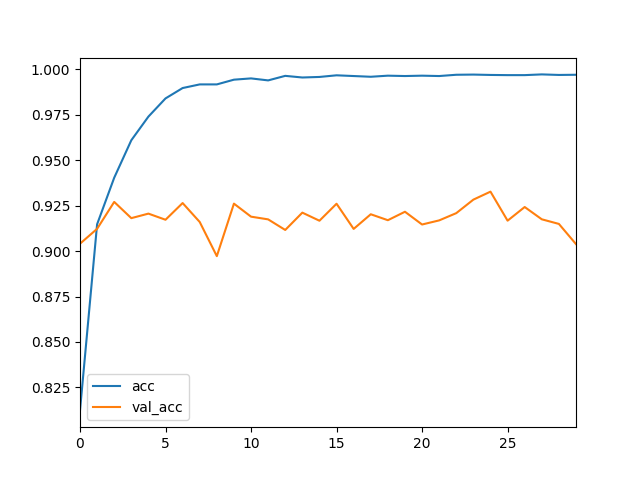
\includegraphics[width=9cm]{zipf_acc.png} }}%
    \subfloat[Loss]{{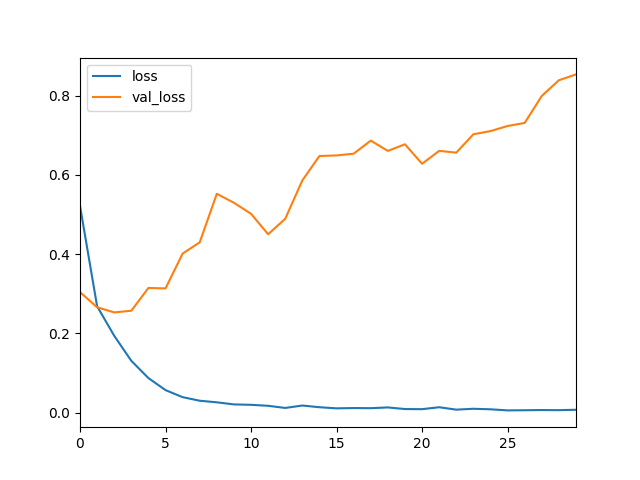
\includegraphics[width=9cm]{zipf_loss.png} }}%
    \caption{Zipf's Law with CNN}%
    \label{fig:example}%
\end{figure}


\begin{center}
\subsection{Final Results}
\end{center}

For this project we tried four different approaches: using a combination of TF-IDF, MLOGIT, GloVe vectors, and CNN.
The overall accuracy for each approach can be found in table \ref{table_acc_overall}. When visualing these url embeddings we see great results. We can observe that for the most part each category is clustered together. 
\newpage
\subsubsection{Accuracy Results}

\begin{table}[ht!]
\centering
\begin{tabular}{l|l}
model & accuracy \\
\hline
GloVe \& MLOGIT & 89.5\% \\
TF-IDF \& MLOGIT & 90.5\%  \\
GloVe \& CNN & 92.1\%  \\
GloVe \& Zipf's Law \& CNN & 93.2\%  \\
\end{tabular}
\caption{Accuracy results for all of our approaches}
\label{table_acc_overall}
\end{table}

\subsubsection{Semantic Results}

\begin{figure}[ht!]
\center
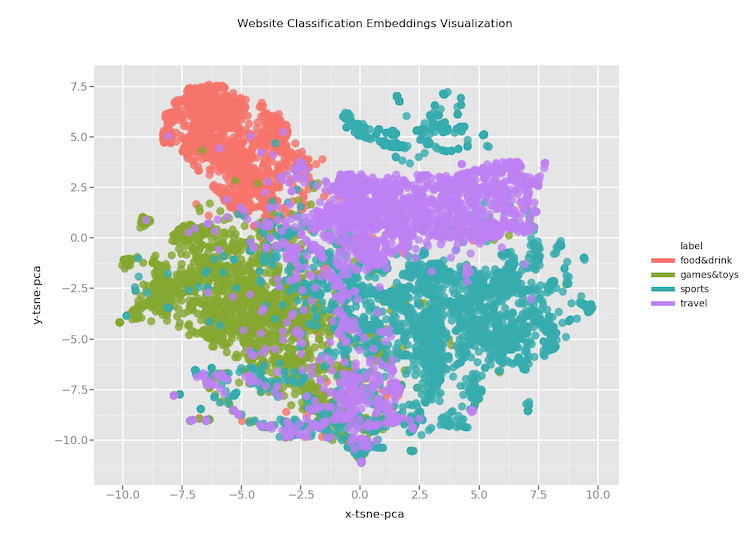
\includegraphics[width=110mm]{visual.png}
    \caption{Website Embeddings}
    \label{glove_vectors}
\end{figure}


\subsubsection{Binary Results}
To make a more fair comparison with works discussed in Chapter 2, we decided to binarize the data. We want to detect if the website is a sports site or not. We decided with this category because it is the class with the most instances. We get a fairly balanced data set with 5,860 non-sport sites and 4,766 sport sites.

\begin{table}[ht!]
\centering
\begin{tabular}{l|l}
model & accuracy \\
\hline
GloVe \& LOGIT & 94.2\% \\
TF-IDF \& LOGIT & 93.4\%  \\
GloVe \& CNN & 94.6\%  \\
GloVe \& Zipf's Law \& CNN & 94.8\%  \\
\end{tabular}
\caption{Binary Accuracy results for all of our approaches}
\label{binary_results}
\end{table}

\newpage
\section*{
\begin{center}
CHAPTER 5 
\end{center}
\newline 
\begin{center}
CONCLUSION
\end{center}}

\setcounter{subsection}{0}
\addtocounter{section}{1}

Overall one can see that the most complex model - the CNN - with Zipf's Law performed the best. It is important to note that websites with small sample of words will not follow Zipf's distribution and therefore not perform as expected. Additionally, this is in agreement with previous work which suggests that feature extraction methods help improve downstream machine learning tasks. Finally, looking at the visualizations we can conclude that these url embeddings capture semantic meaning, where similar websites are close to each other. After we transformed our multiclass classification problem into a binary one, we saw a jump in accuracy. All models got an accuracy of 94\% except for the base model (TF-IDF \& LOGIT), which got a 93\%.

\newpage
\section*{
\begin{center}
CHAPTER 6
\end{center}
\newline 
\begin{center}
FUTURE WORK
\end{center}}

\setcounter{subsection}{0}
\addtocounter{section}{1}

There are a lot ways how our work can be continued and improved.
Having more data can not only help to improve the overfitting problem for the CNN but can also lead to a higher accuracy for the MLOGIT classifiers. The next step would be to clean the data more thoroughly by applying other NLP techniques such as stemming and annotating.

Also the hyperparameters for the CNN model and Zipf's Law should be fine tuned more in order to improve its performance. Other network architectures such as Recurrent Neural Networks or Hierarchical Attention Networks could lead to better results as well. 

Furthermore, it might be a good approach to train our own word embeddings instead of using a pretrained one. By training from scratch on our dataset the model will be more fitted to our specific tasks and potentially produce better results.


Finally, concatenating different word embeddings may help improve model accuracy. This approach can inject complementary information from diverse word embeddings, which helps generalize the representations. It can be viewed as a type of ensemble learning.



%-------------------------------Appendix-----------------------------------
\newpage
\begin{appendices}
	\sections {Zipf's Law - Python}
	\centering

\begin{verbatim}
'''
    File name: zipfs.py
    Author: Alejandro Robles
    Objective: Preprocess text using Zipf's Law
    Python Version: 3.6
'''
from pandas import DataFrame
from math import pow
from collections import Counter
from nltk.corpus import stopwords
from langdetect import detect
import numpy as np

class Zipf:
    target_column = ''
    vector_column = 'Counter_Text'
    output_column = 'Clean_Text'

    def __init__(self, q=2, lower=True):
        self.q = q
        self.lower = lower

    def fit(self, dataframe, target_column='Text'):
        self.target_column = target_column
        self.dataframe = dataframe

    def transform(self, output_column='Clean_Text'):
        self.output_column = output_column
        self._vectorize()
        self._cleanText()

    def filter_by_language(self, lang='en', col_name=None):
        if col_name:
            coltarget=col_name
        else:
            coltarget=self.target_column

        bool_index = [False] * self.dataframe.shape[0]
        for i, text in enumerate(self.dataframe[coltarget]):
            try:
                bool_index[i] = detect(text) == lang
            except:
                pass
        self.dataframe = self.dataframe.loc[bool_index]

    def _vectorize(self):
        clean_text = []
        if self.lower:
            self.dataframe[self.target_column] = self.dataframe[self.target_column].str.lower()
        for text in self.dataframe[self.target_column]:
            try:
                temp = Zipf.getJ1(text, self.q, True)
            except:
                temp = []
            clean_text.append(temp)
        self.dataframe[self.vector_column] = clean_text

    def _cleanText(self):
        clean_text = []
        for text_vector in self.dataframe[self.vector_column]:
            try:
                words = self.get_strings(text_vector)
                no_stops = self.remove_stopwords(words)
                clean_row = ' '.join(no_stops)
            except:
                clean_row = np.nan
            clean_text.append(clean_row)
        self.dataframe[self.output_column] = clean_text

    @staticmethod
    def getK(q, n=3):
        return (pow(q, n) - 1) / (q - 1)
        
    @staticmethod
    def getJ(arr, q, n=3):
        c = arr.sum()
        k = Zipf.getK(q, n)
        j2 = c / k
        j1 = j2 * q
        j0 = j1 * q
        return [j0, j1, j2]
        
    @staticmethod
    def findindex(arr, value):
        return (np.abs(arr.cumsum() - value)).argmin()
        
    @staticmethod
    def getIndices(arr, j):
        range0 = Zipf.findindex(arr, j[0]) + 1
        range1 = Zipf.findindex(arr[range0 + 1:], j[1]) + 1
        return [(0, range0), (range0, range0 + range1), (range0 + range1, len(arr))]
        
    @staticmethod
    def getSubset(arr, tup):
        return arr[tup[0]:tup[1]]
        
    @staticmethod
    def checkCard(arr, indices):
        subs = [Zipf.getSubset(arr, ind) for ind in indices]
        lens = [len(sub) for sub in subs]
        return subs, lens

    @staticmethod
    def getJ1(text, q, split=False):
        words_dict = Zipf.get_counter(text, split)
        word_counts = np.array([word[1] for word in words_dict])
        j = Zipf.getJ(word_counts, q)
        s = Zipf.getIndices(word_counts, j)
        return Zipf.getSubset(words_dict, s[1])

    @staticmethod
    def get_counter(words, split=False):
        if split:
            words = words.split()
        return Counter(words).most_common()

    @staticmethod
    def get_strings(arr, index=0):
        return [w[index] for w in arr]

    @staticmethod
    def remove_stopwords(words):
        return [word for word in words if word not in stopwords.words('english')]

if __name__ == '__main__':
    path = 'files/scrapedsites.json'
    df = getData(path)
    z = Zipf(q=2)
    z.fit(df)
    z.transform()
\end{verbatim}
\end{appendices}

\newpage
\printbibliography

\end{document}